\documentclass{beamer}

\usepackage{Vor2018glærur}

\title{Tölvunarfræði 2}
\subtitle{Vika 9}

\begin{document}

\begin{frame}
	\titlepage
\end{frame}

\section{Inngangur}

\section{Praktísk atriði}

\subsection{Aflúsun}

\begin{frame}{Aflúsun}
	\begin{columns}
		\column{0.5\textwidth}
		\begin{itemize}
			\item Aflúsun \eng{debugging} vísar til þess almenna ferlis að ``finna villur'' í forriti
			      \begin{itemize}
				      \item Upphaflega mjög bókstaflegt
				      \item Í dag - búum til og skoðum logga, framkvæmum einingaprófanir, fylgjumst með kerfisástandi,\ldots
			      \end{itemize}
			\item Skoðum notkun á sérhæfðum aflúsurum \eng{debuggers}
		\end{itemize}
		\column{0.5\textwidth}
		\begin{center}
			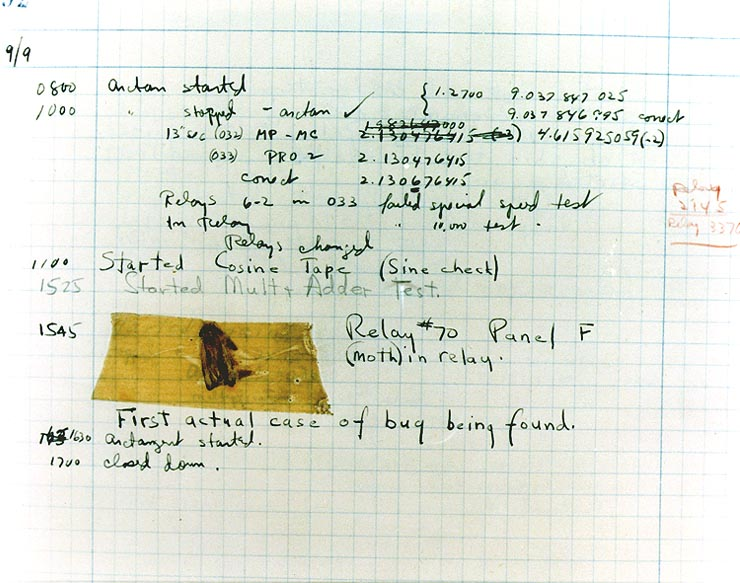
\includegraphics[width=\textwidth]{../T1a/Pics/first-bug}
		\end{center}
	\end{columns}
\end{frame}

\begin{frame}{Aflúsarar}
	\begin{itemize}
		\item Aflúsari er forrit sem notað er til að finna villur í forritskóða
		\item Í dag - aflúsarar fyrir algeng forritunarmál byggð inn í ritla
		      \begin{itemize}
			      \item Forritið er þá þýtt og keyrt í sérstökum aflúsunarham
		      \end{itemize}
		\item Eiginleikar sem við ættum að sjá í flestum aflúsurum:
		      \begin{itemize}
			      \item Breakpoint - staður í forriti merktur með ``punkti''. Þegar forritið er keyrt í aflúsunarham stöðvar forritið keyrslu á þessum stað. Þá má skoða gildi allra breyta á þessum stað í keyrslu forritsins.
			      \item Continue - forritið keyrt fram að næsta breakpoint
			      \item Step over - farið í næstu línu í keyrslu forritsins, hoppað yfir fallsköll
			      \item Step into - farið í næstu línu í keyrslu forritsins,
			            kafað inn í fallsköll
			      \item Step out - farið út úr núverandi fallskalli
		      \end{itemize}
	\end{itemize}
\end{frame}

\begin{frame}{Aflúsun í VS Code}
	\begin{itemize}
		\item Skoðum aflúsun á C++ kóða í Visual Studio Code
		      \begin{itemize}
			      \item Hugmyndirnar eru eins í öðrum ritlum og forritunarmálum
		      \end{itemize}
		\item Breakpoint skilgreindur með því að smella vinstra megin við línunúmer í ritlinum
		\item Þá má nota stjórntækin (eða flýtilykla) til að framkvæma aðgerðir:
		      \begin{center}
			      
\includegraphics{vs-code-debug-buttons}
		      \end{center}
		      Continue, step over, step into, step out, restart og stop
		\item Aflúsunartól í VS Code þurfa uppsetningu, sjá \href{https://code.visualstudio.com/Docs/editor/debugging}{leiðbeiningar}
	\end{itemize}
\end{frame}

\imageslide{vs-code-breakpoint}

\subsection{Uppsetning Java verkefna}

\begin{frame}{Uppsetning Java-verkefna}
	\begin{columns}
		\column{0.5\textwidth}
		\begin{itemize}
			\item Java-forrit hafa fastmótaða uppbyggingu
			\item Til að Java-forritsskrá sé rétt skilgreind þarf hennar í skráarkerfinu (mappan) að passa við \texttt{package} skilgreiningu hennar
			\item Kunnuglegt dæmi:\\ \texttt{\scriptsize package edu.princeton.cs.algs4;}
		\end{itemize}
		\column{0.5\textwidth}
		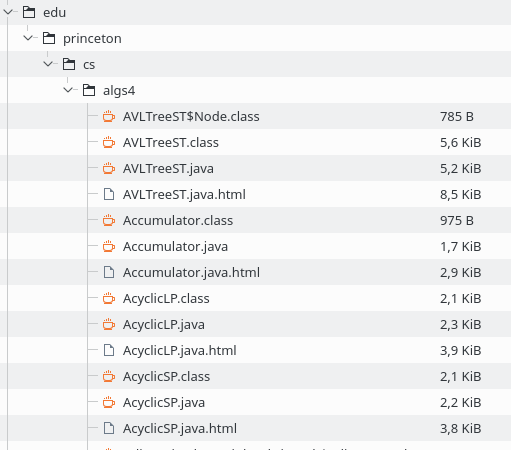
\includegraphics[width=\linewidth]{algs4-package}
	\end{columns}
\end{frame}

\begin{frame}[fragile]{Þýðingardæmi}
	Skrárnar \texttt{Hello.java} og \texttt{HelloWithPackage.java} eru eins fyrir utan \texttt{package} línuna og staðsetningu þeirra. Séum við stödd í möppunni w9 virkar eftirfarandi:

	\begin{minted}[fontsize=\small, frame=lines]{bash}
w9$ javac Hello.java && java Hello
Halló heimur!
w9$ javac is/hi/HelloPackage.java && java is/hi/HelloPackage
Halló heimur!
\end{minted}
	En eftirfarandi virkar ekki þó við séum stödd í w9/is/hi:
	\begin{minted}[fontsize=\small, frame=lines]{bash}
w9/is/hi$ javac HelloPackage.java && java Hellopackage
Error: Could not find or load main class Hellopackage
\end{minted}
\end{frame}

\begin{frame}[fragile]{Classpath}
	\begin{itemize}
		\item \texttt{import} skipanir er hægt að nota til að fá aðgang að klösum í öðrum pökkum
		\item En til þess þarf Java-keyrsluumhverfið að vita hvar hægt er að finna klasana
		      \begin{itemize}
			      \item Hægt að gera það með möppustrúktúrnum (sjá \texttt{UsingPackage.java})
			      \item Einnig hægt að láta keyrsluumhverfið vita sérstaklega hvar klasa má finna
		      \end{itemize}
		\item Keyrsluumhverfið leitar að klösum á stað sem kallaður er ``classpath''
		\item Getum stillt classpath með því að stilla \texttt{CLASSPATH} kerfisbreytuna eða \texttt{-cp} valkostinn þegar forritið er keyrt
	\end{itemize}
\end{frame}

\section{Minnisuppröðun og hlutbundin forritun}

\begin{frame}[fragile]{Minnisuppröðun}
	\begin{columns}
		\column{0.4\textwidth}
		\cppfile[firstline=8, lastline=11, label=Node.c, linenos=false, fontsize=\small]{Code/w9/Node.c}
		\column{0.6\textwidth}
		\begin{itemize}
			\item Í forritunarmálinu C (fyrirrennara C++) eru engir klasar
			\item Getum búið til \texttt{struct} til að halda utan um breytur
			\item Þetta hjálpar okkur að raða upp minni
		\end{itemize}
	\end{columns}
\end{frame}

\begin{frame}{Hlutbundin forritun}
	\begin{itemize}
		\item Töluverð hugmyndafræði fylgir hlutbundinni forritun, en við höfum notað hana sem viðbót við þau tól sem við höfum til að skipuleggja minni
		      \begin{itemize}
			      \item Höfum búið til nýjar gagnagrindur sem ekki voru fyrir í málinu!
		      \end{itemize}
		\item Aðferðir \eng{methods} í klösum Java og C++ klösum gefa okkur sérstaklega mikla möguleika
	\end{itemize}
\end{frame}

\begin{frame}{Lykilorðið \texttt{static}}
	\begin{itemize}
		\item Í Java tilheyra allar aðferðir klösum, líka \texttt{main} aðferðir
		\item Þurfum að ákvarða hvort að aðferðir sem við búum til tilheyri \emph{klasa} eða \emph{tilviki af klasa}
		      \begin{itemize}
			      \item Tilviksaðferðir \eng{instance methods} tilheyra tilviki, er sjálfgefið
			      \item Klasaaðferðir \eng{class methods} tilheyra klasa
		      \end{itemize}
		\item Tilsvarandi á við um eiginleika klasa \eng{class properties}
		\item Dæmi um klasa með mörgum klasaaðferðum: \href{https://docs.oracle.com/javase/8/docs/api/java/lang/Math.html}{\texttt{Math}}
	\end{itemize}
\end{frame}

\begin{frame}{Dæmi}
	\javafile[firstline=3, lastline=21, fontsize=\scriptsize, label=StaticExample.java]{Code/w4/StaticExample.java}
\end{frame}

\section{Eintengdir listar}

\begin{frame}[fragile]{Eintengdur listi}
	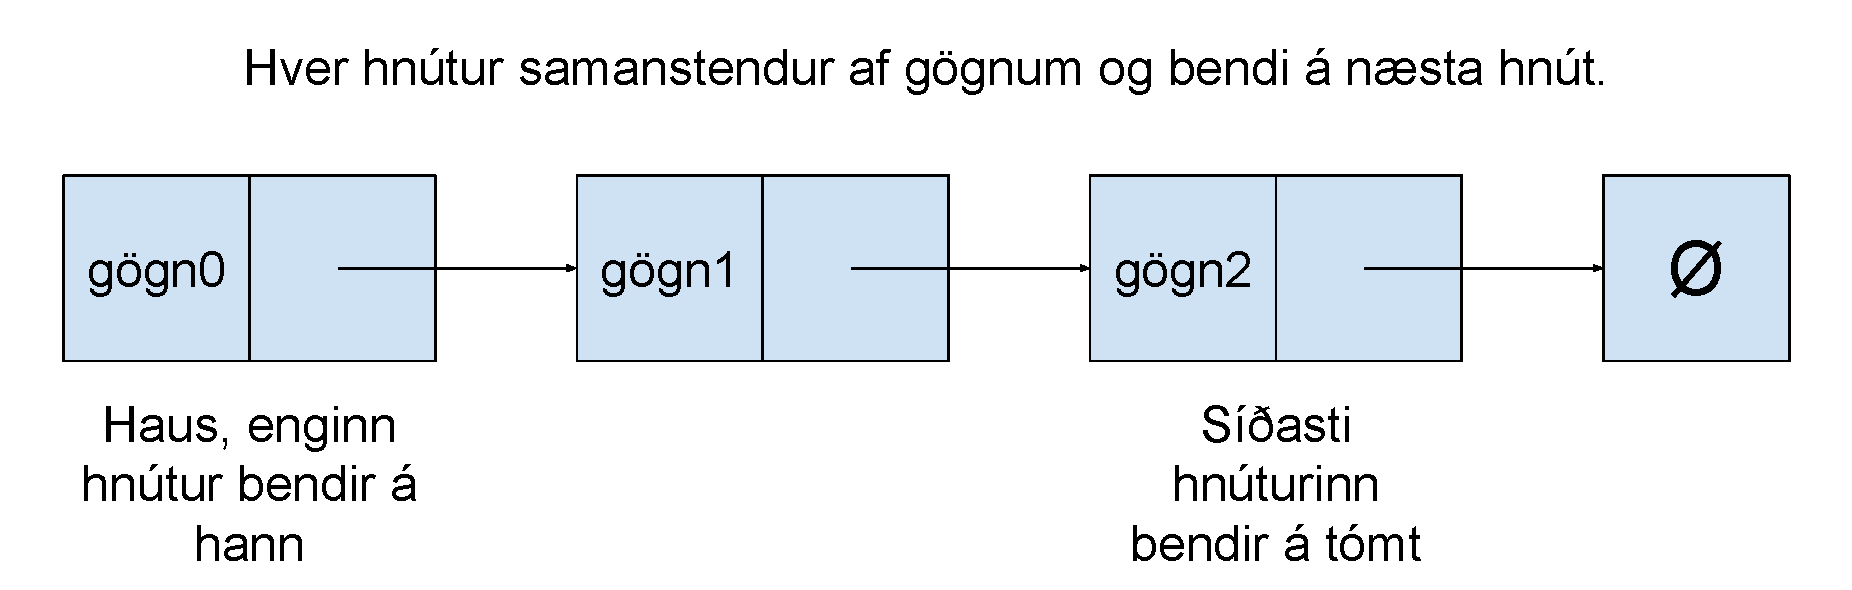
\includegraphics[width=\textwidth]{singly-linked-list}

	\begin{columns}
		\column{0.3\textwidth}
		\begin{minted}[frame=lines, label=Í java]{java}
class Node {
    Node next;
    int data;
}
		\end{minted}
		\column{0.3\textwidth}
		\begin{minted}[frame=lines, label=Í C++]{cpp}
class Node {
    Node* next;
    int data;
}
\end{minted}

	\end{columns}
\end{frame}

\begin{frame}[fragile]{Klasi til að halda utan um hnúta}
	\javafile[firstline=5, lastline=21, fontsize=\scriptsize, label=SinglyLinkedList.java]{Code/w9/SinglyLinkedList.java}
\end{frame}

\begin{frame}[fragile]{Hnút bætt við framan á lista}
	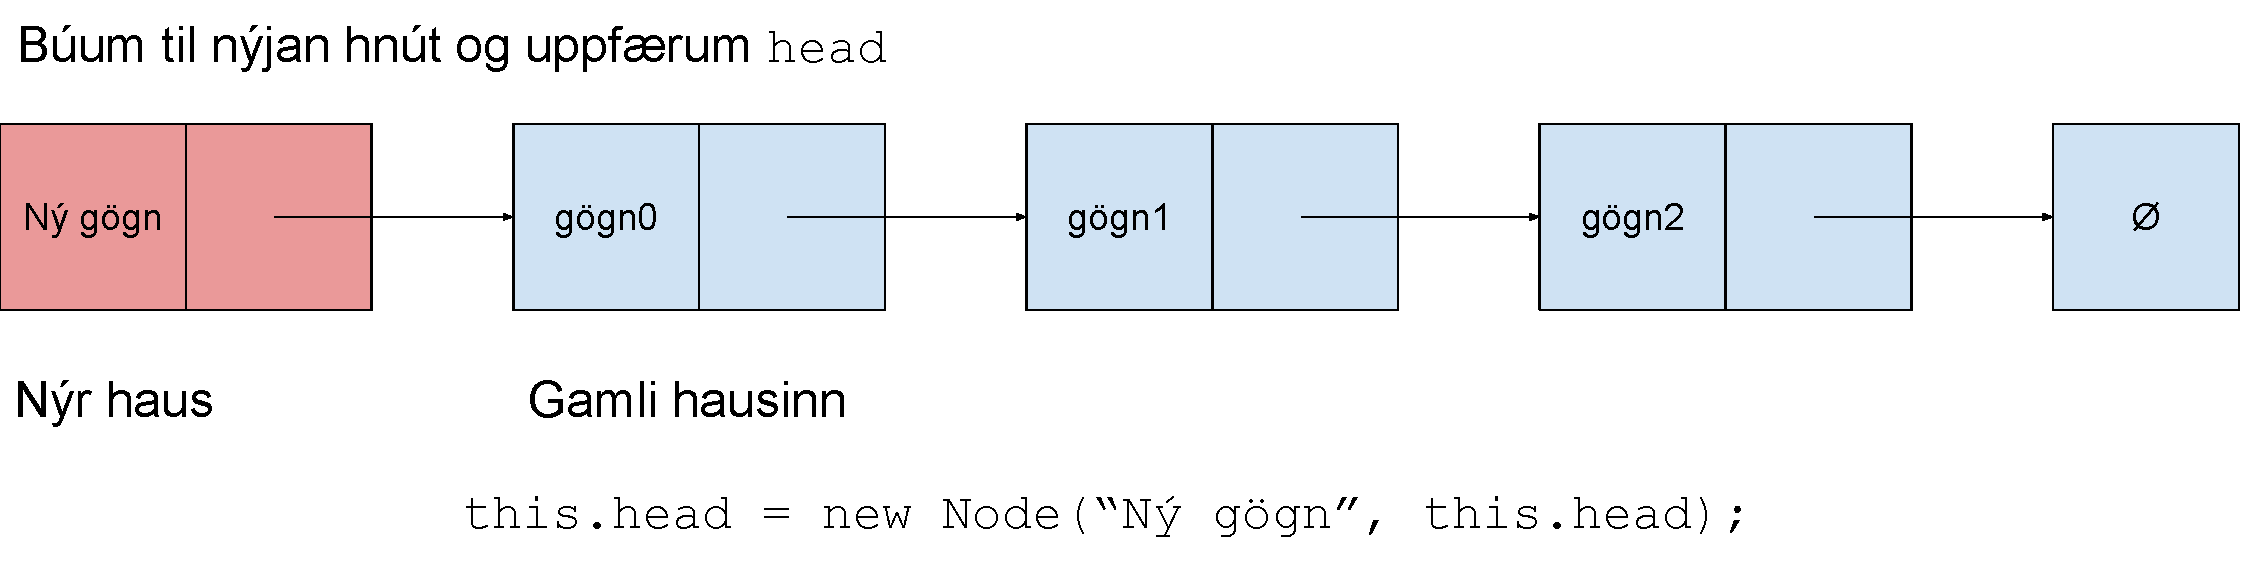
\includegraphics[width=\textwidth]{singly-linked-list-prepend}
\end{frame}

\begin{frame}[fragile]{Hnút bætt við í lista}
	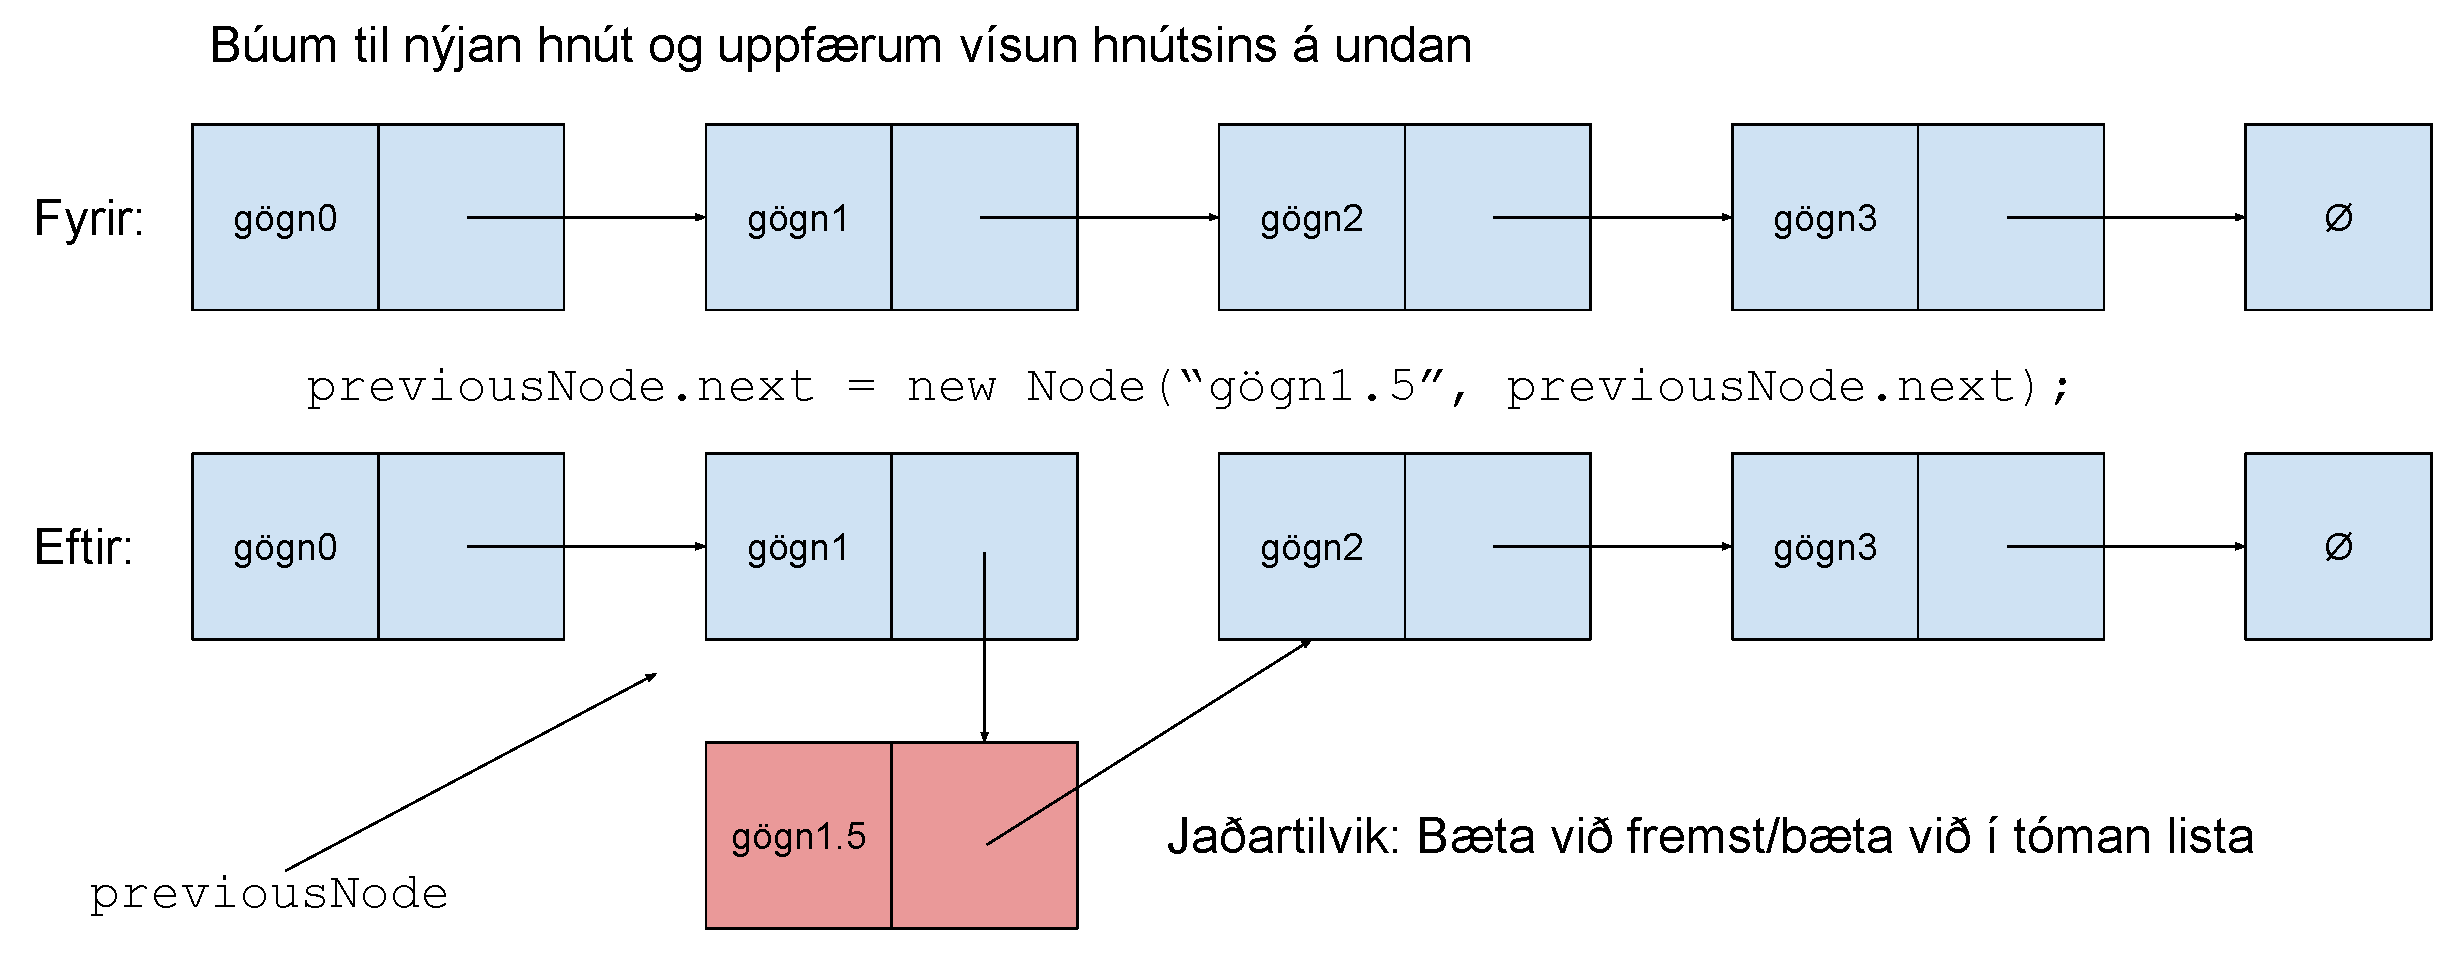
\includegraphics[width=\textwidth]{singly-linked-list-insert}
\end{frame}

\begin{frame}[fragile]{Hnútur fjarlægður úr lista}
	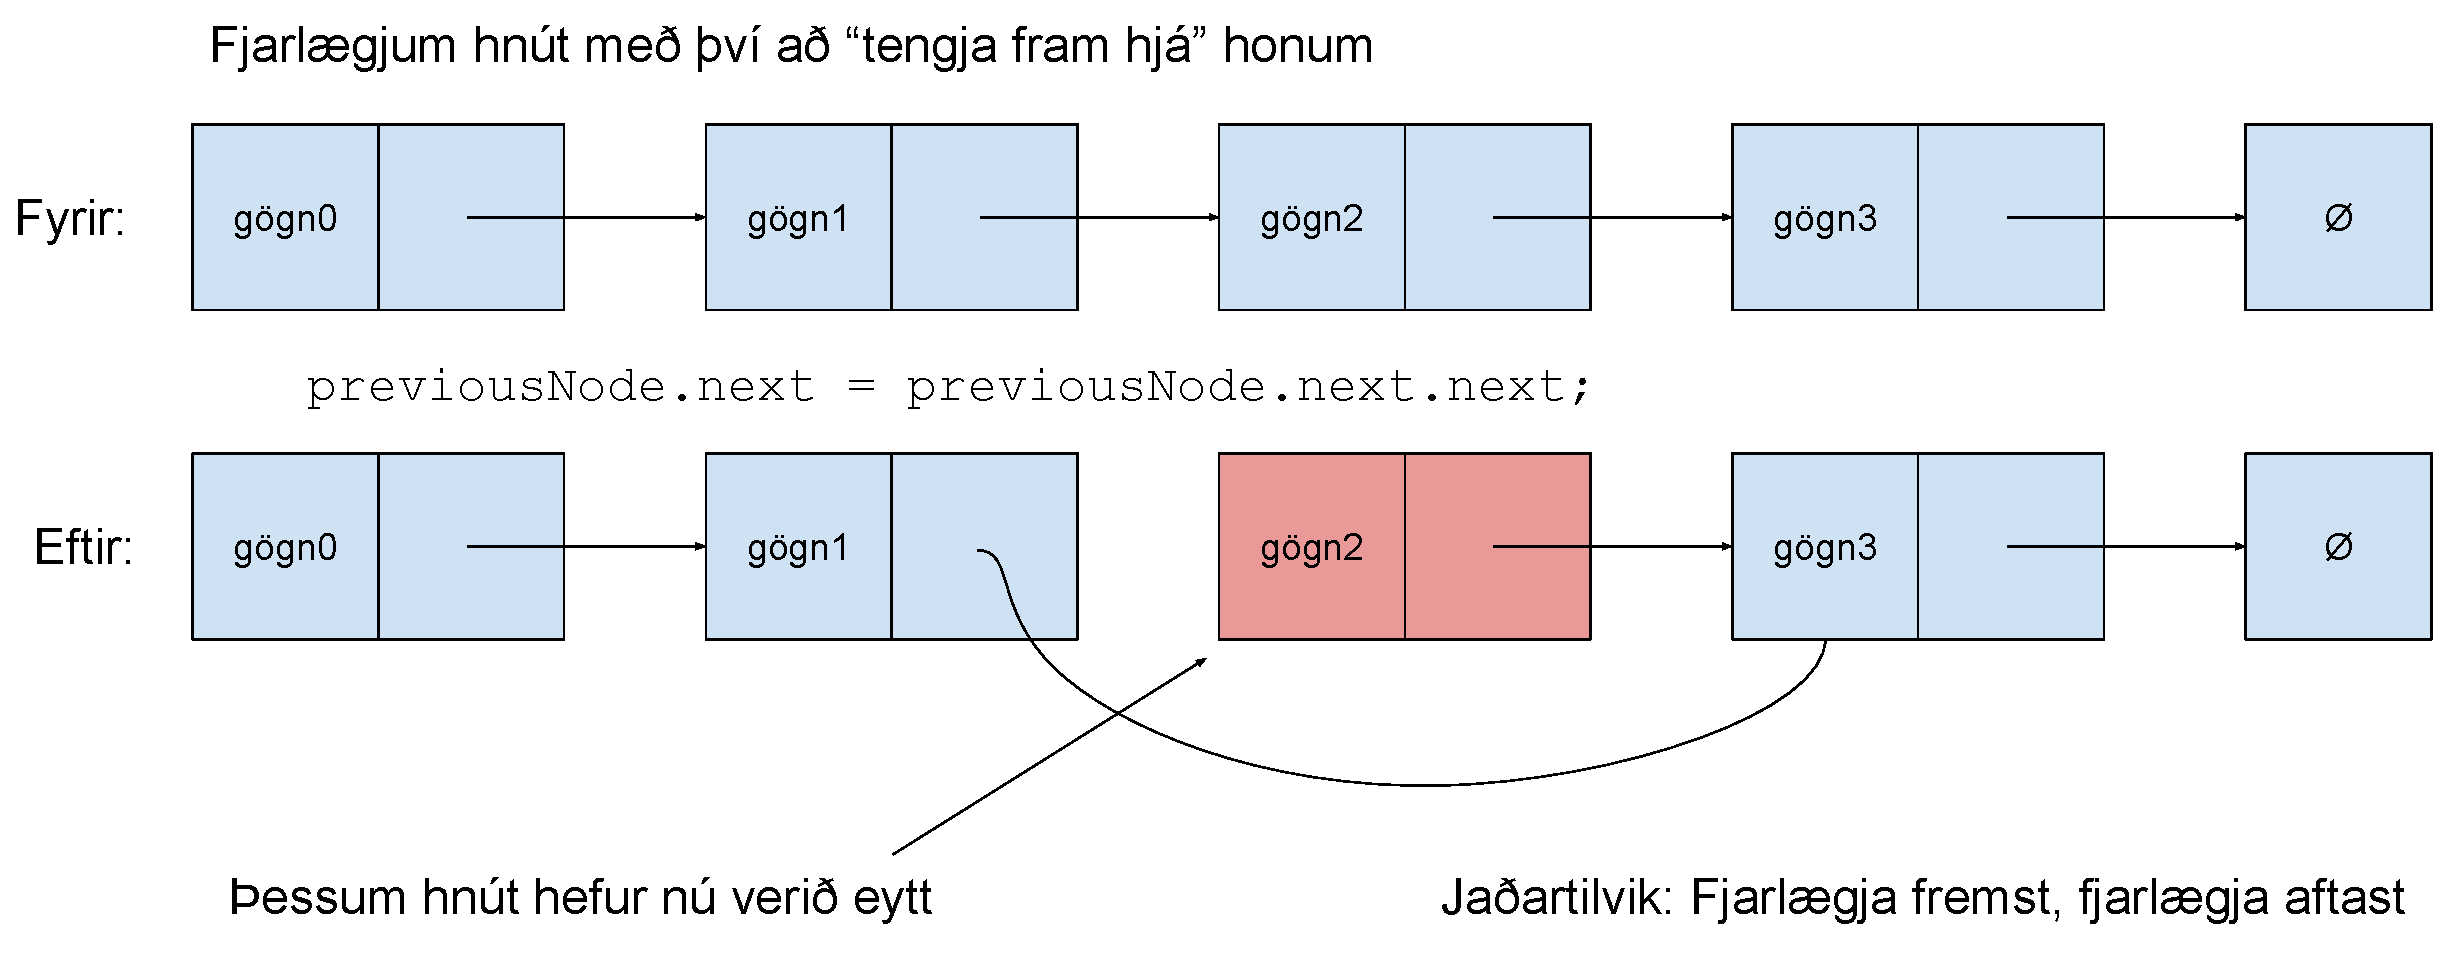
\includegraphics[width=\textwidth]{singly-linked-list-delete}
\end{frame}

\begin{frame}[fragile]{Hnútur fjarlægður úr lista}
	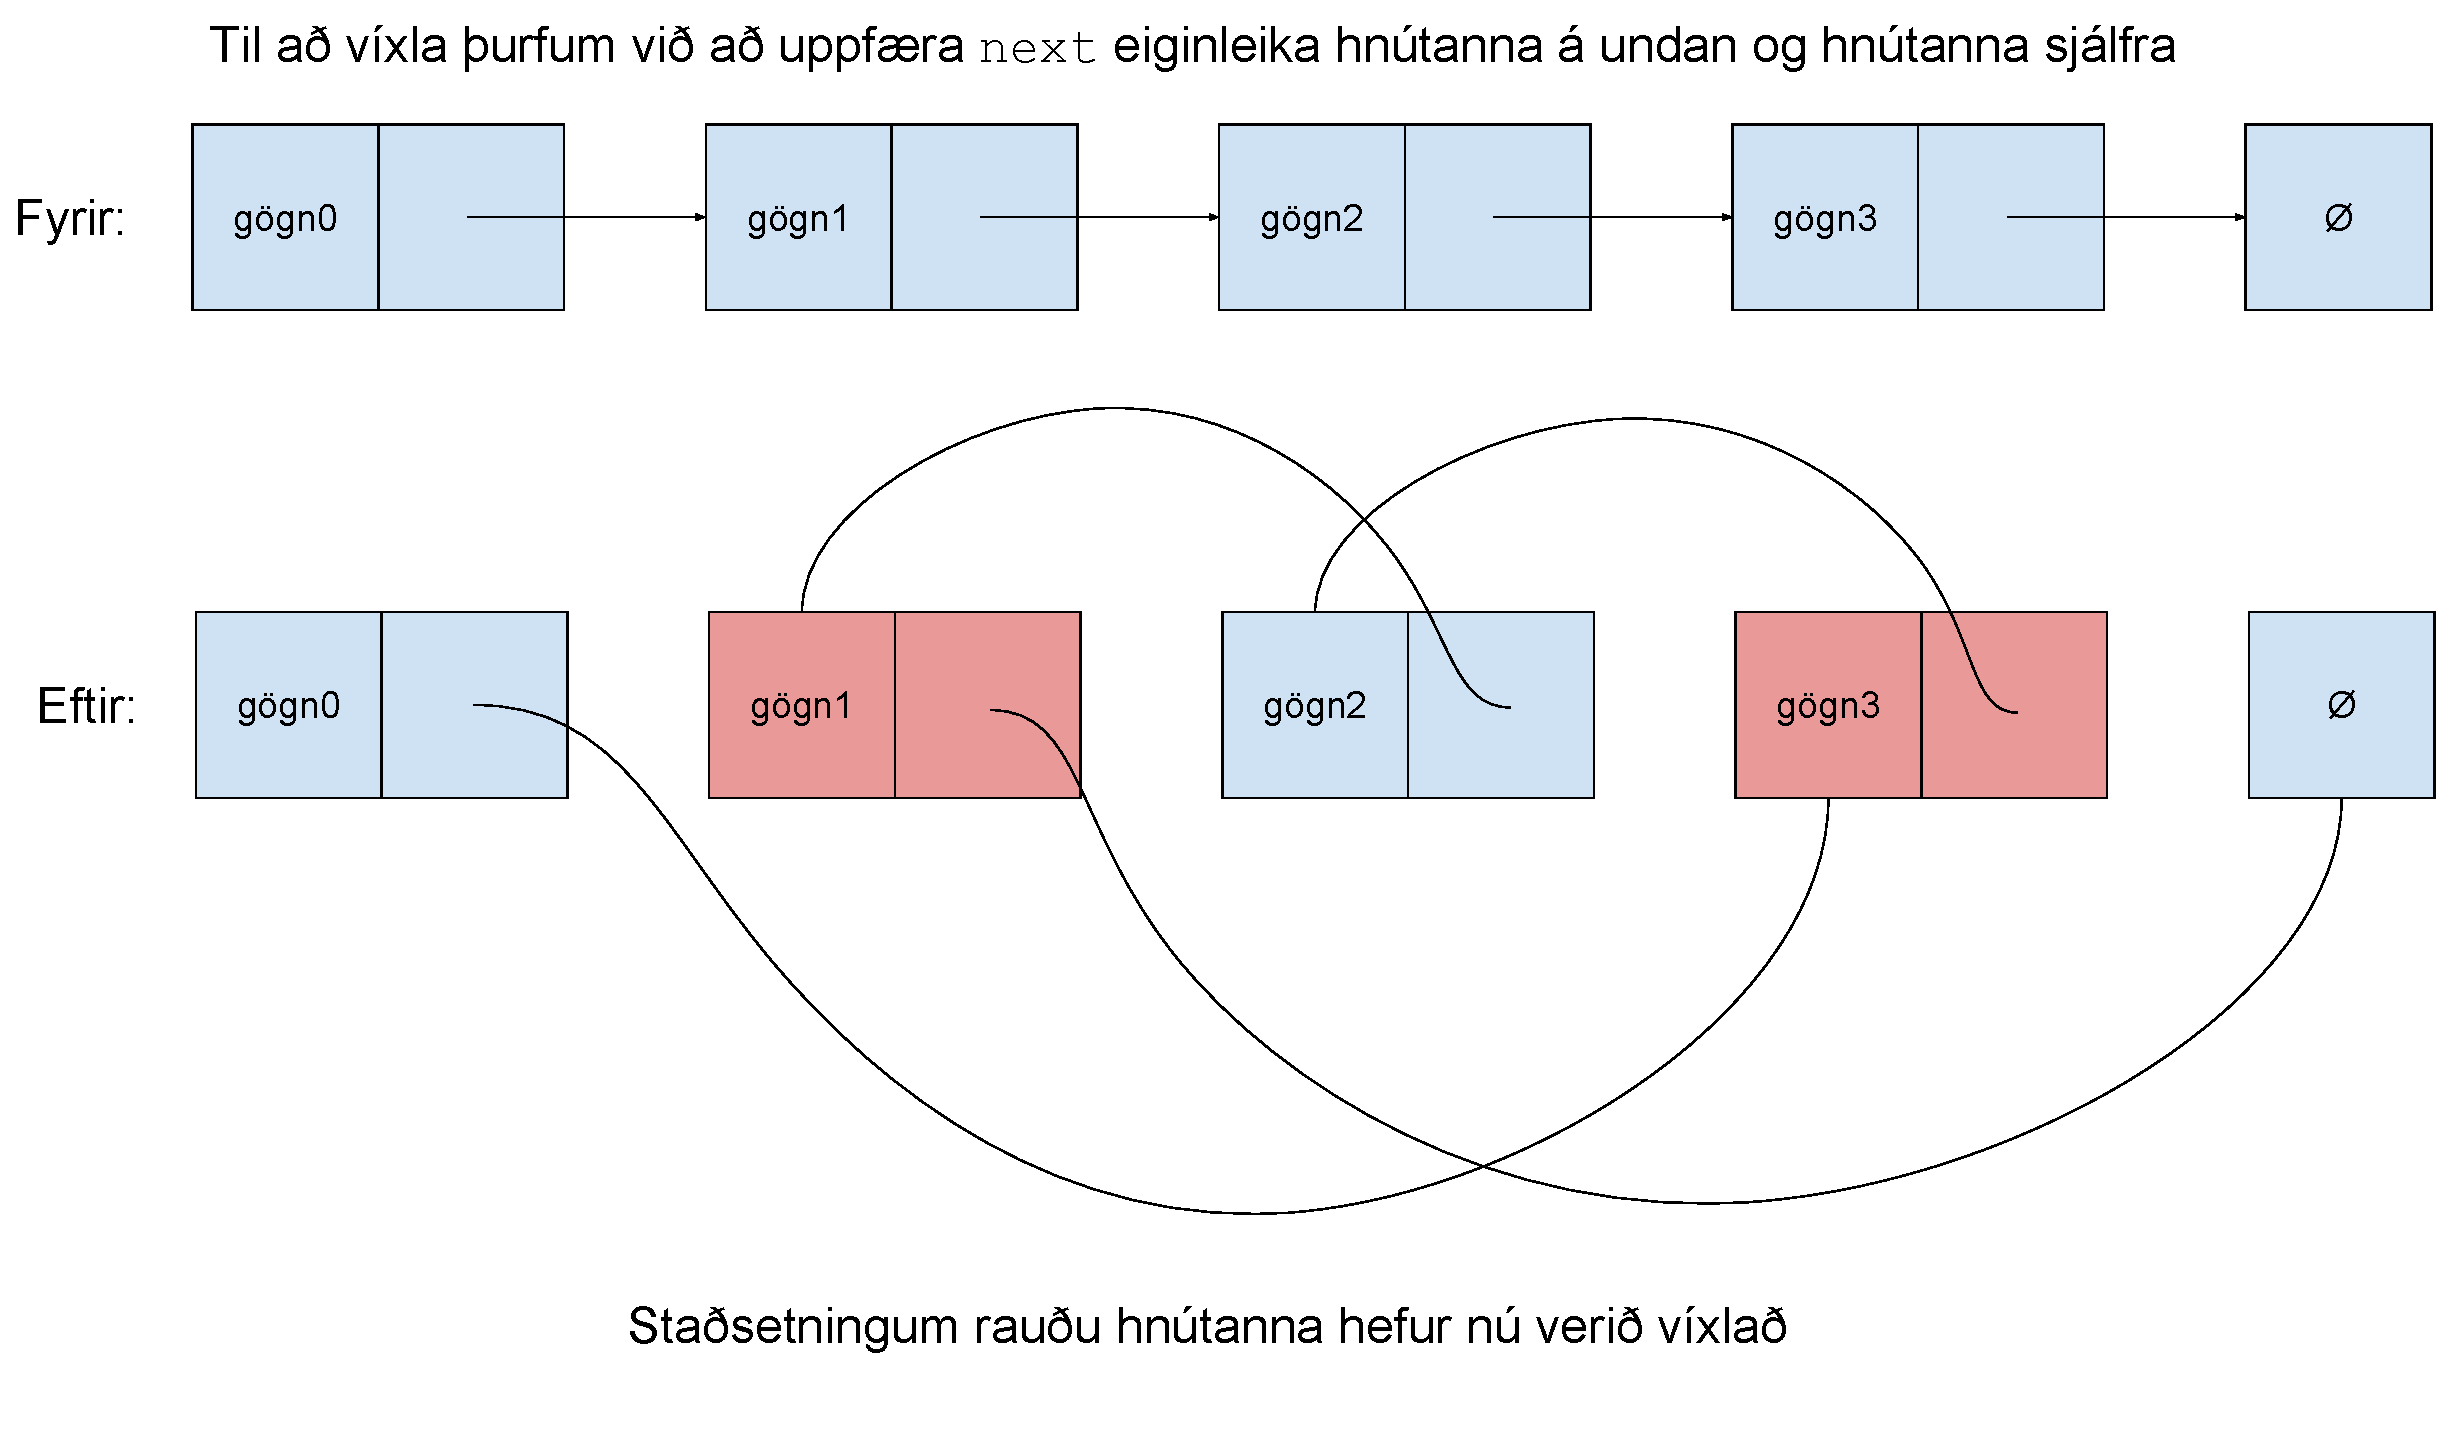
\includegraphics[width=\textwidth]{singly-linked-list-swap}
\end{frame}

\begin{frame}{Næst}
	Meira um tvíleitartré (kafli 3.3) og hakkatöflur (kafli 3.4).
\end{frame}

\end{document}
